\documentclass[11pt]{article}
% STUDENTS:
% You can enter your solutions into this template by just
% typing them right after it says "SOLUTION".
% Ignore the \ifdefined\sol blocks; you can delete them if you want.
% (Note that it won't compile if you try to uncomment the
% solution flag :))
%
% Problem set: do not define TEMPLATE or SOL
% LaTeX template: define TEMPLATE but not SOL
% Solution: define both TEMPLATE and SOL
%
% \def\sol{1}
% \def\template{1}
\usepackage{fullpage,graphicx}
\usepackage{amsmath,amsfonts,amsthm,amssymb,multirow, url}
\usepackage{tikz}
\usetikzlibrary{shapes.symbols}
\usepackage{wrapfig}
\usepackage{algorithmic}
\usepackage{enumerate}
\usepackage{wasysym}
\usepackage{framed}
\usepackage{float}
\usepackage[ruled,vlined,commentsnumbered,titlenotnumbered]{algorithm2e}
\newcommand{\expecting}[1]{\noindent{[\textbf{We are expecting:} \em #1\em]}}
\newcommand{\pts}[1]{\textbf{(#1 pt.)}}
\newcommand{\hint}[1]{\noindent{[\textbf{Hint:} \em #1 \em]}}
\definecolor{shadecolor}{gray}{0.95}



\begin{document}
\noindent
CS 161 \hfill \textbf{Problem Set 3} \newline 
{Fall 2025} \hfill \textbf{Due:} Friday October 24 at 11:59pm on Gradescope.

\noindent
\rule{\linewidth}{0.4pt}

\noindent
\textbf{Style guide and expectations:} Please see the top of the ``Homework" page on the course webpage for guidance on what we are looking for in homework solutions.  We will grade according to these standards.

Make sure to look at the ``\textbf{We are expecting}'' blocks below each problem to see what we will be grading for in each problem!
\newline\newline
\textbf{Collaboration policy:} You may do the HW in groups of size up to three.  Please submit one HW for your whole group on Gradescope.  (Note that there is an option to submit as a group).  See the ``Policies'' section of the course website for more on the collaboration policy.
\noindent
\newline\newline
\textbf{LLM policy:} Check out the course webpage for best practices on how to productively use LLMs on homework, if you use them at all.   \newline\noindent
\rule{\linewidth}{0.4pt}

\section*{Exercises}
We recommend you do the exercises on your own before collaborating with your group.  The point is to check your understanding.

\noindent
\rule{\linewidth}{0.4pt}
\begin{enumerate}

%%%%%%%%%%%%%% EXERCISE 1 %%%%%%%%%%%%%%%%%%%%%%%%%


\item \pts{6}
In this exercise, we'll explore different types of randomized algorithms.  We say that a randomized algorithm is a \textbf{Las Vegas Algorithm} if it is always correct, but the running time is a random variable.  We say that a randomized algorithm is a \textbf{Monte Carlo Algorithm} if there is some probability that it is incorrect.  For example, QuickSort (with a random pivot) is a Las Vegas algorithm, since it always produces a sorted array (but if we get very unlucky QuickSort may be slow).  

Suppose that there is a population of $n$ ducks.  Half of the ducks are green, and half are brown, but it's dark outside and you can't tell the difference until you catch one and look at it with a flashlight.  Assume that catching a random duck and looking at it takes time $O(1)$.

The algorithms given in Figure~\ref{algs} all attempt to find a single green duck. 
Fill in the chart below.  You may use asymptotic notation for the running times; give the best big-Oh bound that you can.  For the probability of returning a correct duck, do not use asymptotic notation; give the best bound that you can.
\begin{center}
\begin{tabular}{|c|p{3cm}|p{2cm}|p{2cm}|p{4cm}|}
\hline
Algorithm & Monte Carlo or Las Vegas? & Expected running time 
& Worst-case running time & Probability of returning a green duck \\
\hline
\textbf{Algorithm 1} &  &  &  & \\
\hline
\textbf{Algorithm 2} &  &  &  & \\
\hline
\textbf{Algorithm 3} &  &  &  & \\
\hline
\end{tabular}
\end{center}
Note that the \LaTeX \ code for the table is available in the source file.

\hint{Remember (see Lecture 5 and the pre-lecture exercise) that the expectation of a geometric random variable with probability $p$ is equal to $\frac{1}{p}$}

\expecting{A filled-in table.  No justification is required.}

\begin{figure}[h]
\begin{algorithm}[H]
\KwIn{A flock of $n$ ducks}
\While{true}
{
Choose a random duck from the flock\;
\If{That duck is green}{ \Return{ that duck } }
\Else{Release the duck back into the flock}
}
\caption{\textsc{findGreenDuck1}}
\end{algorithm}

\begin{algorithm}[H]
\KwIn{A flock of $n$ ducks}
\For{100 iterations}
{
Choose a random duck from the flock\;
\If{That duck is green}{ \Return{ that duck } }
\Else{Release the duck back into the flock}
}
Choose a random duck from the flock\;
\Return{ That duck }
\caption{\textsc{findGreenDuck2}}
\end{algorithm}

\begin{algorithm}[H]
\KwIn{A flock of $n$ ducks}
Put the ducks in a line, in a random order \;
\tcc{Assume it takes time $O(n)$ to put the $n$ ducks in a random order; and assume that they stay put once ordered.}
\For{ $i = 0, \ldots, n-1$ }
{
\If{Duck $i$ is green}{ \Return{ Duck $i$ } }
}
\caption{\textsc{findGreenDuck3}}
\end{algorithm}
\caption{Three algorithms for finding a green duck}\label{algs}
\end{figure}\clearpage

\ifdefined\template
\begin{shaded}
\textbf{SOLUTION:}

\ifdefined\sol
\input{solutions/E1.tex}
\fi
\end{shaded}
\fi


%%%%%%%%%%%%% Exercise 2 %%%%%%%%%%%%%%%%%%%%%

\item {\pts{4} [\textbf{Coloring RB Trees.}] }
	
	Can you color in the nodes of the trees below to make legitimate red-black trees? For each tree, either color the nodes to make a valid red-black tree, or say that no such coloring exists.  
 
 \textbf{Note:} the \LaTeX\ code to make these trees is included in the template.  If you'd like to use this code, you can color a node by editing it like: 
 
 \verb|\node[draw,circle,fill=red]| or \verb|\node[draw,circle,fill=black]|.  
 
 Or you can just color the nodes in your favorite drawing program and include the image with \verb|\includegraphics{my_image.png}|.
    
    \begin{center}
    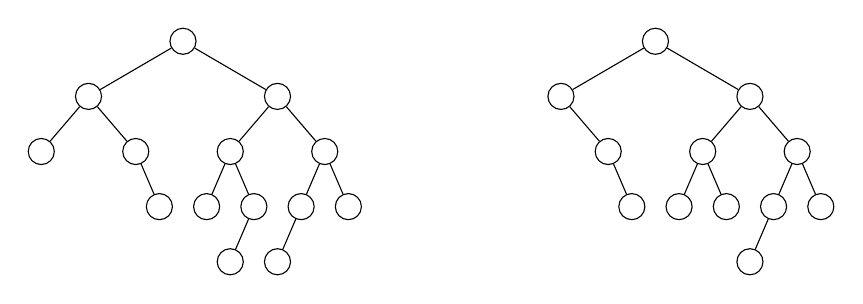
\begin{tikzpicture}[xscale=0.6,yscale=.7]
    \begin{scope}
    \node[draw,circle](b) at (0,0) {};
    \node[draw,circle](b0) at (-2,-1) {};
    \node[draw,circle](b1) at (2,-1) {};
    \node[draw,circle](b00) at (-3,-2) {};
    \node[draw,circle](b01) at (-1,-2) {};
    \node[draw,circle](b10) at (1,-2) {};
    \node[draw,circle](b11) at (3,-2) {};
    
    \node[draw,circle](b011) at (-0.5,-3) {};
    \node[draw,circle](b100) at (0.5,-3){};
    \node[draw,circle](b101) at (1.5,-3){};
    \node[draw,circle](b110) at (2.5,-3) {};
    \node[draw,circle](b111) at (3.5,-3) {};
    
    \node[draw,circle](b1010) at (1,-4) {};
    \node[draw,circle](b1100) at (2,-4) {};

    
    \draw (b) -- (b0);
    \draw (b) -- (b1);
    \draw (b0) -- (b00);
    \draw (b0) -- (b01);
    \draw (b1) -- (b10);
    \draw (b1) -- (b11);
    \draw (b01) -- (b011);
    \draw (b10) -- (b100);
    \draw (b10) -- (b101);
    \draw (b11) -- (b110);
    \draw (b11) -- (b111); 
    \draw (b110) -- (b1100);
    \draw (b101) -- (b1010);
    \end{scope}
    
    \begin{scope}[xshift=10cm]
    \node[draw,circle](b) at (0,0) {};
    \node[draw,circle](b0) at (-2,-1) {};
    \node[draw,circle](b1) at (2,-1) {};
    \node[draw,circle](b01) at (-1,-2) {};
    \node[draw,circle](b10) at (1,-2) {};
    \node[draw,circle](b11) at (3,-2) {};
    
    \node[draw,circle](b011) at (-0.5,-3) {};
    \node[draw,circle](b100) at (0.5,-3){};
    \node[draw,circle](b101) at (1.5,-3){};
    \node[draw,circle](b110) at (2.5,-3) {};
    \node[draw,circle](b111) at (3.5,-3) {};
    
    \node[draw,circle](b1100) at (2,-4) {};
    
    \draw (b) -- (b0);
    \draw (b) -- (b1);
    \draw (b0) -- (b01);
    \draw (b1) -- (b10);
    \draw (b1) -- (b11);
    \draw (b01) -- (b011);
    \draw (b10) -- (b100);
    \draw (b10) -- (b101);
    \draw (b11) -- (b110);
    \draw (b11) -- (b111);
    \draw (b110) -- (b1100);
    \end{scope}
    \end{tikzpicture}
    \end{center}
    
    \expecting{For each tree, either an image of a colored-in red-black tree or a statement ``No such red-black tree.''  No justification is required.}

\ifdefined\template
\begin{shaded}
\textbf{SOLUTION:}

\ifdefined\sol
\input{solutions/E2.tex}
\fi
\end{shaded}
\fi

%%%%%%%%%%%%%%%%%% EXERCISE 3 %%%%%%%%%%%%%%%%%%%%%%%%%%%

\item\pts{5} This exercise references the IPython notebook \texttt{HW3.ipynb}, available on the course website along with this problem set.

In our implementation of radixSort in class, we used bucketSort to sort each digit.  Why did we use bucketSort and not some other sorting algorithm?  There are several reasons,  and we'll explore one of them in this exercise.

\begin{enumerate}
\item\pts{2} One reason we chose bucketSort was that it makes radixSort work correctly!  In \texttt{HW3.ipynb}, we've implemented four different sorting algorithms---bucketSort, quickSort, and two versions of mergeSort---as well as radixSort.  

\textbf{Note:} The IPython notebook is long, but just because it implements many different sorting algorithms.  Don't get scared!  

There is a \texttt{TODO} statement in the IPython notebook where you can change the code to use different sorting algorithms; you just have to make sure that the sorting algorithm you want to use is the one that is not commented out.  No programming necessary!

Modify the code for radixSort to use each one of these four algorithms within radixSort, and test it out on the examples suggested.

Which sorting algorithms seem to be correct as ``inner sorting algorithms'' for radixSort? 
\begin{itemize}
    \item Does using bucketSort always work correctly?
    \item Does using quickSort always work correctly?
    \item Does using mergeSort (with merge1) always work correctly?
    \item Does using mergeSort (with merge2) always work correctly?
\end{itemize}
\expecting{Yes or no for each part.}
\item\pts{3} Explain what you saw above.  What was special about the algorithms which worked?  Why does this special thing matter?  (You may wish to play around with \texttt{HW3.ipynb} to ``debug" the incorrect cases.)

\expecting{A clear definition of the special property that the correct algorithms have, and a few sentences explaining why it matters.
A minimal example of what might go wrong is a great way to explain why this property matters.

You do not need to justify 
why each of the algorithms do or do not have the property. }

Note: yes, this property is alluded to in the reading.  That's why this is an exercise and not a problem!  To get the most out of this exercise, play around with the examples in the code and make sure you really understand what's going on.

\end{enumerate}
\ifdefined\template
\begin{shaded}
\textbf{SOLUTION:}

\ifdefined\sol
\input{solutions/E3.tex}
\fi
\end{shaded}
\fi


\end{enumerate}
\newpage
\section*{Problems}

\noindent
\rule{\linewidth}{0.4pt}

\begin{enumerate}
\setcounter{enumi}{3}
%%%%%%%%%%%%%%%%%%%%%%%%%%%%% Problem 4:  Duck Politics  %%%%%%%%%%%%%%%%%%%%%%
\item \pts{6} \textbf{[Ducks.]}
Suppose that $n$ ducks are standing in a line.  
\begin{center}
\includegraphics[width=2cm]{duck}
\hspace{.1cm}
\includegraphics[width=2cm]{duck}
\hspace{.1cm}
\includegraphics[width=2cm]{duck}
\hspace{.1cm}
\includegraphics[width=2cm]{duck}
\hspace{.1cm}
\includegraphics[width=2cm]{duck}
\hspace{.1cm}
\includegraphics[width=2cm]{duck}
\end{center}

Each duck has a political leaning: left, right, or center.  You'd like to sort the ducks so that all the left-leaning ones are on the left, the right-leaning ones are on the right, and the centrist ducks are in the middle.
You can only do two sorts of operations on the ducks:

\begin{center}
\begin{tabular}{|c|c|c|}
\hline
Operation & Result\\
\hline
\texttt{poll(j)} & Ask the duck in position $j$ about its political leanings \\ 
\hline
\texttt{swap(i,j)} & Swap the duck in position $j$ with the duck in position $i$ \\
\hline
\end{tabular}
\end{center}

However, in order to do either operation, you need to pay the ducks to cooperate: each operation costs one piece of duckweed.  Also, you didn't bring a piece of paper or a pencil (or your smartphone or tablet or tablet or whatever you use to take notes) so you can't write anything down and have to rely on your memory!  Like many humans, your memory is limited, and you can only remember up to seven\footnote{\url{https://en.wikipedia.org/wiki/The_Magical_Number_Seven,_Plus_or_Minus_Two}} integers between $0$ and $n-1$ at a time (i.e. you can use at most seven integer-valued variables at a time in your algorithm).

Design an algorithm to sort the ducks, which costs $O(n)$ pieces of duckweed, and uses no extra memory other than storing at most seven\footnote{You don't need to use all seven storage spots, but you can if you want to.  Can you do it with only two?} integers between $0$ and $n-1$.

\hint{Does this task look like anything we've seen in class?}

\expecting{Pseudocode \textbf{AND} a short English description of your algorithm; \textbf{AND} a short explanation of why it uses only $O(n)$ pieces of duckweed and never uses more than seven numbers of memory.}



\ifdefined\template
\begin{shaded}
\textbf{SOLUTION:}
\ifdefined\sol
\input{solutions/ducks.tex}
\fi
\end{shaded}
\fi

%%%%%%%%%%%%%%%%%%%%%%%%%%%%% Problem 5: Ducks of new heights  %%%%%%%%%%%%%%%%%%%%%%
\newpage
\item \textbf{[Ducks.]} \pts{6}
Suppose that $n$ ducks of distinct heights are standing in a line, ordered from shortest to tallest. 
\begin{center}
\includegraphics[height=2cm]{yardstick}
\includegraphics[width=1.5cm,height=1.2cm]{duck}
\hspace{.1cm}
\includegraphics[width=1.5cm,height=1.7cm]{duck}
\hspace{.1cm}
\includegraphics[width=1.5cm,height=1.9cm]{duck}
\hspace{.1cm}
\includegraphics[width=1.5cm,height=2cm]{duck}
\hspace{.1cm}
\includegraphics[width=1.5cm,height=2.5cm]{duck}
\hspace{.1cm}
\includegraphics[width=1.5cm,height=3cm]{duck}
\end{center}

You have a measuring stick of a certain height, and you would like to identify a duck which is the same height as the stick, or else report that there is no such duck. The only operation you are allowed to perform is \texttt{compareToStick(f)}, where $f$ is a duck (that is, you cannot directly access the heights of each duck). \texttt{compareToStick(f)} returns \texttt{taller} if $f$ is taller than the stick, \texttt{shorter} if $f$ is shorter than the stick, and \texttt{the same} if $f$ is the same height as the stick.  You've still forgotten to bring a paper and a pencil and so you can only store up to seven integers in $\{0,\ldots,n-1\}$ at a time.
And you have to pay a duck one piece of duckweed every time you perform \texttt{compareToStick} on it.

\begin{enumerate}
\item \pts{2} Give an algorithm in this model of computation which either finds a duck the same height as the stick, or else returns ``No such duck," and uses $O(\log(n))$ pieces of duckweed. 

\expecting{Pseudocode \textbf{AND} an English description.  You do not need to justify the correctness or duckweed usage. } 
\item \pts{4} Prove that any algorithm in this model of computation must use $\Omega(\log(n))$ pieces of duckweed.

\expecting{A short but convincing argument.}
\end{enumerate}

\ifdefined\template
\begin{shaded}
\textbf{SOLUTION:}
\ifdefined\sol
\input{solutions/yetmoreducks.tex}
\fi
\end{shaded}
\fi

\newpage
%%%%%%%%%%%%%%%%%%%% PROBLEM 6: Wisdom of geese %%%%%%%%%%%%%%%%%%%%%%

\item  \textbf{[Goose!]} \pts{5} A wise goose has knowledge of an array $A$ of length $n$, such that $A[i] \in \{1,\ldots,k\}$ for all $i$.  (Note that the elements of $A$ are not necessarily distinct). 
You don't have direct access to $A$, but you can ask the wise goose \em any \em yes/no questions about it.  For example, you could ask ``If I remove $A[5]$ and swap $A[7]$ with $A[8]$, would the array be sorted?'' or ``can some geese fly as high as 29,000ft?''

Unlike in the previous problems, this time you did bring a paper and pencil, and your job is to write down all of the elements of $A$ in sorted order.\footnote{Note that you don't have any ability to change the array $A$ itself, you can only ask the wise goose about it.}  The wise goose charges one piece of duckweed per question.\footnote{Despite the name, it turns out that geese also eat duckweed.}
\vspace{-.2cm}

\begin{center}
\begin{tikzpicture}
\node(a) {\includegraphics[width=2cm]{alice}};
\node[rotate=-2](b) at (8,.5) {\includegraphics[width=3cm]{wisegoose}};
\node[draw, cloud, cloud puffs=20.5, cloud ignores aspect] at (11,2.5) {$A = [6,2,4,3,3,5,2,1,2,6]$};
\node(c) at (3,2.8) {Is $7$ in the array?};
\node(d) at (5,2) {\textbf{No.}};
\node(e) at (3.5,1) {\begin{minipage}{3.5cm}\begin{center} Do you have tetrachromatic vision?\end{center}\end{minipage}};
\node(f) at (4.5,-.2) {\textbf{Yes.}};
\draw (c) -- (a);
\draw (e) -- (a);
\draw (d) -- (b);
\draw (f) -- (b);
\end{tikzpicture}
\end{center}

\vspace{-.7cm}
\begin{enumerate}
\item\pts{5} Give a procedure that outputs a sorted version of $A$ which uses $O(k\log(n))$ pieces of duck weed.  You may assume that you know $n$ and $k$, although this is not necessary.

\expecting{Pseudocode \text{AND} a short English description of your algorithm; \textbf{AND} a brief explanation of why it uses $O(k \log(n))$ pieces of duckweed.
}
\item \pts{1 BONUS} Prove that any procedure to solve this problem must use $\Omega(k \log(n/k))$ pieces of duckweed. 

\expecting{Nothing; this part is not required.} 
\end{enumerate}

\ifdefined\template
\begin{shaded}
\textbf{SOLUTION:}
\ifdefined\sol
\input{solutions/goose.tex}
\fi
\end{shaded}
\fi


\end{enumerate}



\end{document}
